\documentclass[numbers=noenddot,12pt,a4paper]{scrartcl}
\usepackage[greek,ngerman]{babel}
\usepackage[T1]{fontenc}
\usepackage[utf8]{inputenc}
%\usepackage{ansinew}
\usepackage{fullpage}
\usepackage{libertine}
\usepackage{ziffer}
\usepackage{graphicx}
\usepackage{units}
%\usepackage{wasysym}
\usepackage{amsmath}
\usepackage{amssymb}
\usepackage{wrapfig}
\usepackage{esint}
\usepackage{float}
\usepackage{wrapfig}
\usepackage[font=small]{caption}
\usepackage{subcaption}

\renewcommand{\thefigure}{Abb. \arabic{figure}}

\captionsetup[wrapfigure]{name=}
\captionsetup[figure]{name=}
\newcommand{\degree}{^\circ}
\newcommand{\diff}{\textnormal{d}}
\newcommand{\tenpo}[1]{\cdot 10^{#1}}
\newcommand{\greek}[1]{\greektext#1\latintext}
\newcommand{\ix}[1]{_\text{#1}}
\newcommand{\imag}{\mathbf{i}}
\newcommand{\nicht}[1]{\overline{#1}}

\title{Protokoll: Kombinatorische und sequentielle Schaltungen}
\author{Tom Kranz, Philipp Hacker}
\date{\today}

\begin{document}
%\setcounter{page}{2}
%\setcounter{section}{1}
\maketitle
\vspace*{\fill}
\tableofcontents
\vfill
\newpage
\section{Vorbereitung}
\subsection{Siebensegmentanzeige}
Im Vorfeld des Aufbaus der Siebensegmentanzeige (siehe \ref{img:sieben}) waren durch die Verwendung von Karnaugh-Tafeln die logischen Funktionen der einzelnen Segmente aufzustellen.
\begin{figure}[H]
\begin{minipage}[htbp]{0.28\textwidth}
\centering
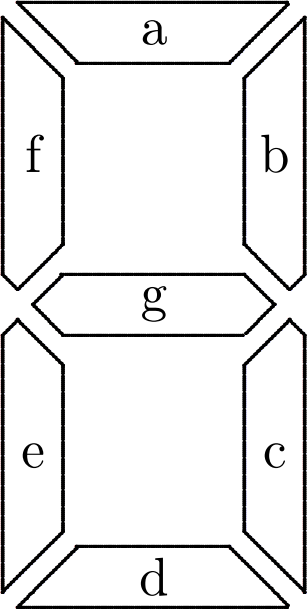
\includegraphics[width=0.65\textwidth]{sieben.png}
\caption{Kennzeichung} \label{img:sieben}
\end{minipage}
\hfill
\begin{minipage}[htbp]{0.68\textwidth}
\begin{table}[H]
\centering
\begin{tabular}{cccc||ccccccc||c}
$x_1$ & $x_2$ & $x_3$ & $x_4$ & a & b & c & d & e & f & g & Anzeige \\ \hline \hline
0 & 0 & 0 & 0 & 1 & 1 & 1 & 1 & 1 & 1 & 0 & 0 \\ 
1 & 0 & 0 & 0 & 0 & 1 & 1 & 0 & 0 & 0 & 0 & 1 \\
0 & 1 & 0 & 0 & 1 & 1 & 0 & 1 & 1 & 0 & 1 & 2 \\
1 & 1 & 0 & 0 & 1 & 1 & 1 & 1 & 0 & 0 & 1 & 3 \\
0 & 0 & 1 & 0 & 0 & 1 & 1 & 0 & 0 & 1 & 1 & 4 \\
1 & 0 & 1 & 0 & 1 & 0 & 1 & 1 & 0 & 1 & 1 & 5 \\
0 & 1 & 1 & 0 & 1 & 0 & 1 & 1 & 1 & 1 & 1 & 6 \\
1 & 1 & 1 & 0 & 1 & 1 & 1 & 0 & 0 & 0 & 0 & 7 \\
0 & 0 & 0 & 1 & 1 & 1 & 1 & 1 & 1 & 1 & 1 & 8 \\
1 & 0 & 0 & 1 & 1 & 1 & 1 & 1 & 0 & 1 & 1 & 9 \\
\end{tabular}
\caption{Wahrheitstabelle der Siebensegmentanzeige} \label{tab:wahr}
\end{table}
\end{minipage}
\end{figure}

\begin{figure}[H]
\begin{minipage}[htbp]{0.49\textwidth}
\begin{table}[H]
\centering
\begin{tabular}{cc||cc|cc|cc|cc}
$x_1$ & $x_2$ & 0 & 0 & 0 & 1 & 1 & 1 & 1 & 0 \\ \cline{0-1} 
$x_3$ & $x_4$ & & & & & & & & \\ \cline{1-10}
0 & 0 & \multicolumn{2}{|c|}{1} & \multicolumn{2}{|c|}{1} & \multicolumn{2}{|c|}{1} & \multicolumn{2}{|c}{0} \\
0 & 1 & \multicolumn{2}{|c|}{1} & \multicolumn{2}{|c|}{$\ast$} & \multicolumn{2}{|c|}{$\ast$} & \multicolumn{2}{|c}{1} \\ 
1 & 1 & \multicolumn{2}{|c|}{$\ast$} & \multicolumn{2}{|c|}{$\ast$} & \multicolumn{2}{|c|}{$\ast$} & \multicolumn{2}{|c}{$\ast$} \\ 
1 & 0 & \multicolumn{2}{|c|}{0} & \multicolumn{2}{|c|}{1} & \multicolumn{2}{|c|}{1} & \multicolumn{2}{|c}{1} \\ 
\end{tabular}
\caption{Segment a}
\end{table}
Logische Funktion:
\begin{align}
a= x_3 x_1  + x_2 + \overline{x_3} \; \overline{x_1}  + x_4
\end{align}
\end{minipage}
\hfill
\begin{minipage}[htbp]{0.49\textwidth}
\begin{table}[H]
\centering
\begin{tabular}{cc||cc|cc|cc|cc}
$x_1$ & $x_2$ & 0 & 0 & 0 & 1 & 1 & 1 & 1 & 0 \\ \cline{0-1} 
$x_3$ & $x_4$ & & & & & & & & \\ \cline{1-10}
0 & 0 & \multicolumn{2}{|c|}{1} & \multicolumn{2}{|c|}{1} & \multicolumn{2}{|c|}{1} & \multicolumn{2}{|c}{1} \\
0 & 1 & \multicolumn{2}{|c|}{1} & \multicolumn{2}{|c|}{$\ast$} & \multicolumn{2}{|c|}{$\ast$} & \multicolumn{2}{|c}{1} \\ 
1 & 1 & \multicolumn{2}{|c|}{$\ast$} & \multicolumn{2}{|c|}{$\ast$} & \multicolumn{2}{|c|}{$\ast$} & \multicolumn{2}{|c}{$\ast$} \\ 
1 & 0 & \multicolumn{2}{|c|}{1} & \multicolumn{2}{|c|}{0} & \multicolumn{2}{|c|}{1} & \multicolumn{2}{|c}{0} \\ 
\end{tabular}
\caption{Segment b}
\end{table}
Logische Funktion:
\begin{align}
b=x_2 x_1 +\overline{x_1}\;\overline{x_2}+\overline{x_3}
\end{align}
\end{minipage}
\end{figure}

\begin{figure}[H]
\begin{minipage}[htbp]{0.49\textwidth}
\begin{table}[H]
\centering
\begin{tabular}{cc||cc|cc|cc|cc}
$x_1$ & $x_2$ & 0 & 0 & 0 & 1 & 1 & 1 & 1 & 0 \\ \cline{0-1} 
$x_3$ & $x_4$ & & & & & & & & \\ \cline{1-10}
0 & 0 & \multicolumn{2}{|c|}{1} & \multicolumn{2}{|c|}{0} & \multicolumn{2}{|c|}{1} & \multicolumn{2}{|c}{1} \\
0 & 1 & \multicolumn{2}{|c|}{1} & \multicolumn{2}{|c|}{$\ast$} & \multicolumn{2}{|c|}{$\ast$} & \multicolumn{2}{|c}{1} \\ 
1 & 1 & \multicolumn{2}{|c|}{$\ast$} & \multicolumn{2}{|c|}{$\ast$} & \multicolumn{2}{|c|}{$\ast$} & \multicolumn{2}{|c}{$\ast$} \\ 
1 & 0 & \multicolumn{2}{|c|}{1} & \multicolumn{2}{|c|}{1} & \multicolumn{2}{|c|}{1} & \multicolumn{2}{|c}{1} \\ 
\end{tabular}
\caption{Segment c}
\end{table}
Logische Funktion:
\begin{align}
c=\overline{\overline{x_3} \; \overline{c_1} \; x_2}
\end{align}
\end{minipage}
\hfill
\begin{minipage}[htbp]{0.49\textwidth}
\begin{table}[H]
\centering
\begin{tabular}{cc||cc|cc|cc|cc}
$x_1$ & $x_2$ & 0 & 0 & 0 & 1 & 1 & 1 & 1 & 0 \\ \cline{0-1} 
$x_3$ & $x_4$ & & & & & & & & \\ \cline{1-10}
0 & 0 & \multicolumn{2}{|c|}{1} & \multicolumn{2}{|c|}{1} & \multicolumn{2}{|c|}{1} & \multicolumn{2}{|c}{0} \\
0 & 1 & \multicolumn{2}{|c|}{1} & \multicolumn{2}{|c|}{$\ast$} & \multicolumn{2}{|c|}{$\ast$} & \multicolumn{2}{|c}{1} \\ 
1 & 1 & \multicolumn{2}{|c|}{$\ast$} & \multicolumn{2}{|c|}{$\ast$} & \multicolumn{2}{|c|}{$\ast$} & \multicolumn{2}{|c}{$\ast$} \\ 
1 & 0 & \multicolumn{2}{|c|}{0} & \multicolumn{2}{|c|}{1} & \multicolumn{2}{|c|}{0} & \multicolumn{2}{|c}{0} \\ 
\end{tabular}
\caption{Segment d}
\end{table}
Logische Funktion:
\begin{align}
d=x_4+x_2\nicht{x_3}+\overline{x_3} \; \overline{x_1}+ x_2 \nicht{x_1}+ \nicht{x_2}x_1x_3
\end{align}
\end{minipage}
\end{figure}

\begin{figure}[H]
\begin{minipage}[htbp]{0.49\textwidth}
\begin{table}[H]
\centering
\begin{tabular}{cc||cc|cc|cc|cc}
$x_1$ & $x_2$ & 0 & 0 & 0 & 1 & 1 & 1 & 1 & 0 \\ \cline{0-1} 
$x_3$ & $x_4$ & & & & & & & & \\ \cline{1-10}
0 & 0 & \multicolumn{2}{|c|}{1} & \multicolumn{2}{|c|}{1} & \multicolumn{2}{|c|}{0} & \multicolumn{2}{|c}{0} \\
0 & 1 & \multicolumn{2}{|c|}{1} & \multicolumn{2}{|c|}{$\ast$} & \multicolumn{2}{|c|}{$\ast$} & \multicolumn{2}{|c}{0} \\ 
1 & 1 & \multicolumn{2}{|c|}{$\ast$} & \multicolumn{2}{|c|}{$\ast$} & \multicolumn{2}{|c|}{$\ast$} & \multicolumn{2}{|c}{$\ast$} \\ 
1 & 0 & \multicolumn{2}{|c|}{0} & \multicolumn{2}{|c|}{1} & \multicolumn{2}{|c|}{0} & \multicolumn{2}{|c}{0} \\ 
\end{tabular}
\caption{Segment e}
\end{table}
Logische Funktion:
\begin{align}
e=x_1+\nicht{x_2} x_3
\end{align}
\end{minipage}
\hfill
\begin{minipage}[htbp]{0.49\textwidth}
\begin{table}[H]
\centering
\begin{tabular}{cc||cc|cc|cc|cc}
$x_1$ & $x_2$ & 0 & 0 & 0 & 1 & 1 & 1 & 1 & 0 \\ \cline{0-1} 
$x_3$ & $x_4$ & & & & & & & & \\ \cline{1-10}
0 & 0 & \multicolumn{2}{|c|}{1} & \multicolumn{2}{|c|}{0} & \multicolumn{2}{|c|}{0} & \multicolumn{2}{|c}{0} \\
0 & 1 & \multicolumn{2}{|c|}{1} & \multicolumn{2}{|c|}{$\ast$} & \multicolumn{2}{|c|}{$\ast$} & \multicolumn{2}{|c}{1} \\ 
1 & 1 & \multicolumn{2}{|c|}{$\ast$} & \multicolumn{2}{|c|}{$\ast$} & \multicolumn{2}{|c|}{$\ast$} & \multicolumn{2}{|c}{$\ast$} \\ 
1 & 0 & \multicolumn{2}{|c|}{1} & \multicolumn{2}{|c|}{1} & \multicolumn{2}{|c|}{0} & \multicolumn{2}{|c}{1} \\ 
\end{tabular}
\caption{Segment f}
\end{table}
Logische Funktion:
\begin{align}
f=x_4 + \nicht{x_2} \; \nicht{x_1} + \nicht{x_2}x_3 + x_3 \nicht{x_1}
\end{align}
\end{minipage}
\end{figure}

\begin{table}[H]
\centering
\begin{tabular}{cc||cc|cc|cc|cc}
$x_1$ & $x_2$ & 0 & 0 & 0 & 1 & 1 & 1 & 1 & 0 \\ \cline{0-1} 
$x_3$ & $x_4$ & & & & & & & & \\ \cline{1-10}
0 & 0 & \multicolumn{2}{|c|}{0} & \multicolumn{2}{|c|}{1} & \multicolumn{2}{|c|}{1} & \multicolumn{2}{|c}{0} \\
0 & 1 & \multicolumn{2}{|c|}{1} & \multicolumn{2}{|c|}{$\ast$} & \multicolumn{2}{|c|}{$\ast$} & \multicolumn{2}{|c}{1} \\ 
1 & 1 & \multicolumn{2}{|c|}{$\ast$} & \multicolumn{2}{|c|}{$\ast$} & \multicolumn{2}{|c|}{$\ast$} & \multicolumn{2}{|c}{$\ast$} \\ 
1 & 0 & \multicolumn{2}{|c|}{1} & \multicolumn{2}{|c|}{1} & \multicolumn{2}{|c|}{0} & \multicolumn{2}{|c}{1} \\ 
\end{tabular}
\caption{Segment g}
\end{table}
Logische Funktion:
\begin{align}
g=  x_3 \nicht{x_2}+ x_2 \nicht{x_3} + x_4 + x_2\nicht{x_1}
\end{align}

\subsection{Schaltskizzen}
\subsection{Dimensionierung}
\section{Durchführung}
\subsection{Messgeräte}
\subsection{Oszillogramme}
\section{Auswertung}
\section{Anhang}
Die originalen Messwert-Aufzeichnungen liegen bei.
\end{document}